\chapter{Deseño e Implementación}

\section{Módulo de Ficheiros}

O módulo de xestión de ficheiros é un do máis importantes e complexos de todo o programa o cal é lóxico tendo en conta que o programa é un editor de ficheiros.

En canto ao deseño, o principal obxetivo é a extensibilidade do mesmo pois, aínda que o programa está centrado na edición de ficheiros PO e son ests os unicos soportados na actualidade, pretendese que o programa sexa capaz de soportar varios tipos de ficheiros nun futuro. Na figura~\ref{fig:dia_class:files} pódese ver o diagrama de clases deste módulo.

\subsection{Implementación Xenérica}
A implementación da clase \lstinline{File} contén propiedeades para conseguir información sobre o nome e path onde está dito ficheiro, ademáis garda estatísticas sobre o número de mensaxes traducidos, sen traducir ou con tradución difusa. Estas estatísticas actualizanse cada vez que se engade ou elimina unha cadea ou cada vez que esta se modifica. Tamén contén un valor booleano que permite saber se o ficheiro foi modificado. Aparte de métodos para engadir e eliminar cadeas, e para conseguir e modificar os metadatos do ficheiro está clase ten un método para gardar o ficheiro e para analizar o ficheiro. O método para gardar~(\lstinline{save}) emprega o patrón \emph{Template Method\footnote{\href{http://gl.wikipedia.org/wiki/Template_Method_\%28patr\%C3\%B3n_de_dese\%C3\%B1o\%29}{Template Method (patrón de deseño)}}} o cal permitenos actualizar o estado do ficheiro a non cambiado.

Un ficheiro contén instancias de mensaxes~(\lstinline{Message}). As mensaxes teñen como propiedades un estado, orixes, e consellos. A API provee métodos para conseguir e modificar tanto as cadeas orixinais como as traducións na súa forma en singular ou nalgunha das formas plurais. A implementación do método para modificar unha tradución tamén emprega o patrón Template Method para actualizar o estado da mensaxe. Esta clase tamén ten métodos para engadir e eliminar consellos e para obter o contexto da mensaxe.

\begin{figure}[h!]
    \centering
    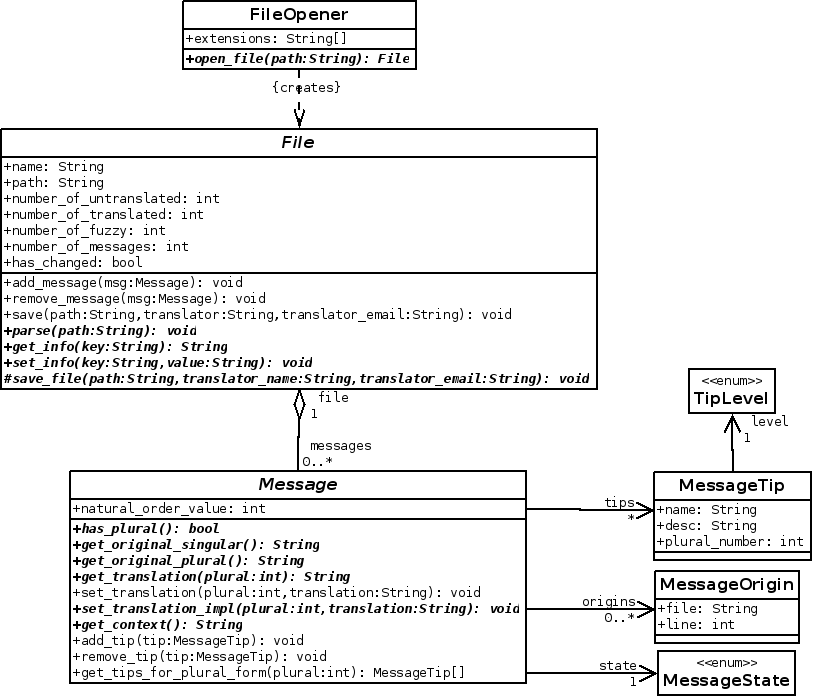
\includegraphics[width=\textwidth]{img/genericfile.png}
    \caption{Diagrama de Clases do módulo ficheiros}
    \label{fig:dia_class:files}
\end{figure}

Ademais a clase \lstinline{FileOpener} recolle un método para crear ficheiros e un conxunto de extensións que se poden abrir con este FileOpener.

\subsubsection{Consellos (Tips)}
Os consellos son a solución que damos para aportar información ao usuario sobre a tradución que está a realizar. Algunha das cousas que pode axudar a indicar esta característica é se a tradución está a ser demasiado longa, se hai algunha palabra que está mal escrita na tradución ou se non emprega a terminoloxía adecuada.

Cada consello ten un nome que debe ser xenerico a cada clase de consello, unha descripción que ten que explicar o problema con detalle, un nivel que indica a gravidade do consello e unha referencia a forma plural a que corresponde dito consello. Ademáis pode conter un ou máis referencias a localización exacta do problema que permitirá destacala na interface gráfica.

A creación de consellos faráse ao modificarse unha cadea e farase a través de plugins.

\subsubsection{Pistas (Hints)}
As pistas amosaranlle ao usuario posibles traducións ou aproximacións as traducións. Estas pistas poden ser obtidas de memorias de traducións, de traducións do mesmo ficheiro noutra linguaxe, ou da tradución directa por exemplo.

Cada instancia dunha pista~(\lstinline{Hint}) contén a tradución suxerida, unha cadea que identifica a orixe de dita pista e un valor que indica a precisión de dita suxerencia.

De igual forma que no caso dos consellos a creación de pistas correrá ao cargo de plugins creados a tal proposito. Neste caso actualizaranse as pistas de cada mensaxe ao selecionalo mesmo na interface.

\subsection{Ficheiro PO}
A implementación especifica para ficheiros PO extende as clases \lstinline{File}, \lstinline{FileOpener} e \lstinline{Message} abstractas para implementar os metodos e permitir empregar ficheiros PO.

Para a analise e a actualización dos ficheiros PO empregaremos a biblioteca gettext-po. No momento no que se iniciou a implementación deste módulo non existía implementación destal librería en Vala polo que tivemos que crear uns \emph{bindings} para poder empregala.

Tanto a clase PoFile como a clase PoMessage delegan a maior parte dos seus métodos nas instancias das clases dos bindings da biblioteca GettextPo File e Message respectivamente. Desta forma faise un claro uso do patrón \emph{Adapter\footnote{\href{http://gl.wikipedia.org/wiki/Adapter_\%28patr\%C3\%B3n_de_dese\%C3\%B1o\%29}{Adapter (patrón de deseño)}}}.

De forma adicional a clase PoFile contén unha instancia da clase PoHeader esta clase que extende e PoMessage correspondese aos metadatos que se atopan nos ficheiros PO na tradución da cadea baleira. É ten meodos para obter e modificar metadatos e para actualizar os datos dos autores das traducións de dito ficheiro. A clase PoFile delega nesta clase a hora de conseguir e modificar metadatos e tamén cando garda un ficheiro.

A clase \lstinline{PoFileOpener} so é capaz de abrir ficheiros con extensión PO e simplemente emprega o método parse da clase ficheiro para crear unha nova instancia.

\subsubsection{Implementación dos bindings}



\section{Módulo de Linguaxes}

\section{Interface Gráfica}

\subsection{Evolución}

\subsection{Paneis}

\begin{figure}[h!]
  \centering
    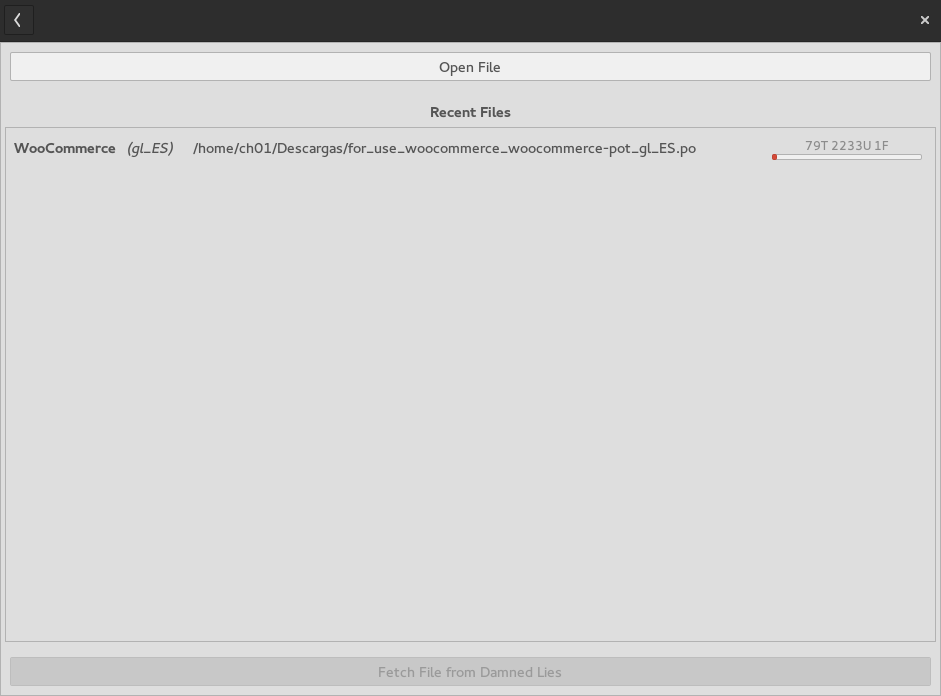
\includegraphics[width=\textwidth]{img/panel_abrir_ficheiro.png}
    \caption{Diagrama de Clases do módulo ficheiros}
    \label{fig:dia_class:files}
\end{figure}

\begin{figure}[h!]
    \centering
    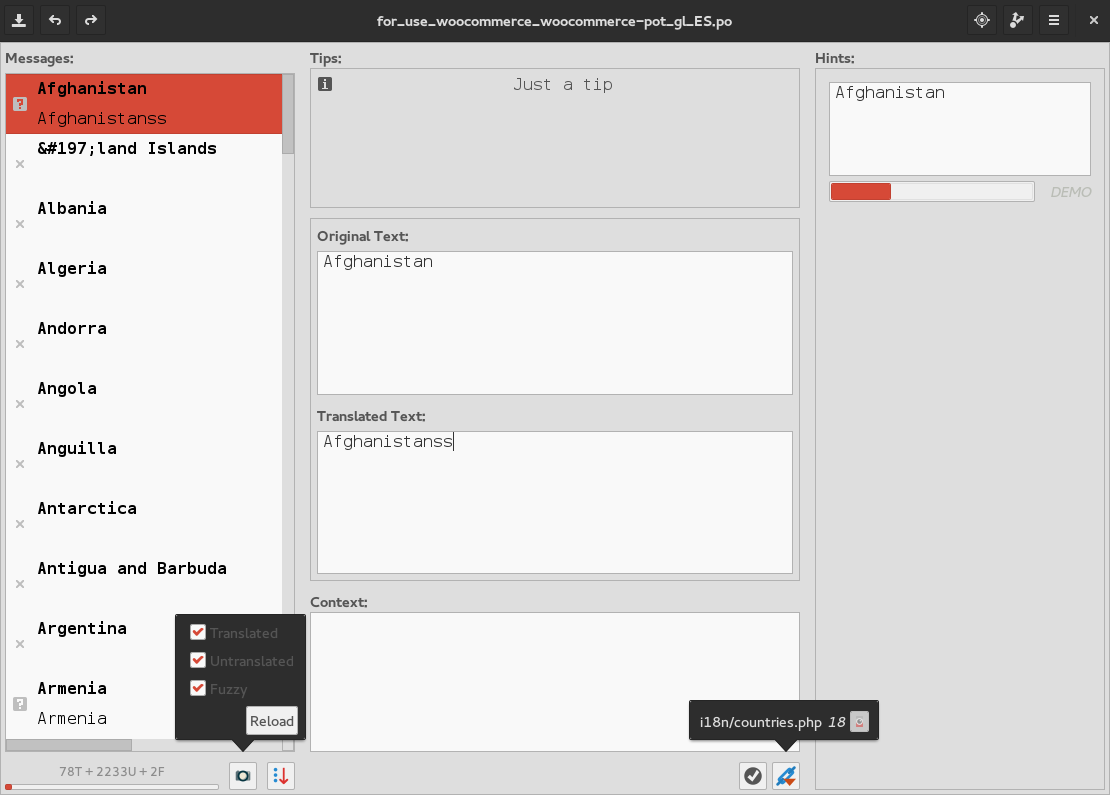
\includegraphics[width=\textwidth]{img/panel_edicion.png}
    \caption{Diagrama de Clases do módulo ficheiros}
    \label{fig:dia_class:files}
\end{figure}

\begin{figure}[h!]
    \centering
    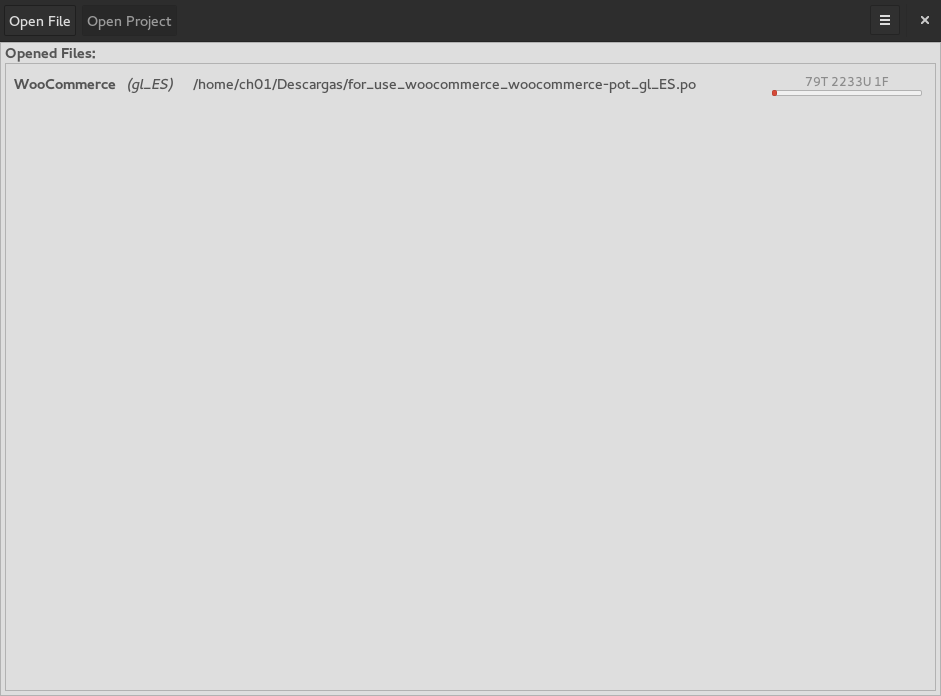
\includegraphics[width=\textwidth]{img/panel_ficheiros_abertos.png}
    \caption{Diagrama de Clases do módulo ficheiros}
    \label{fig:dia_class:files}
\end{figure}

\begin{figure}[h!]
    \centering
    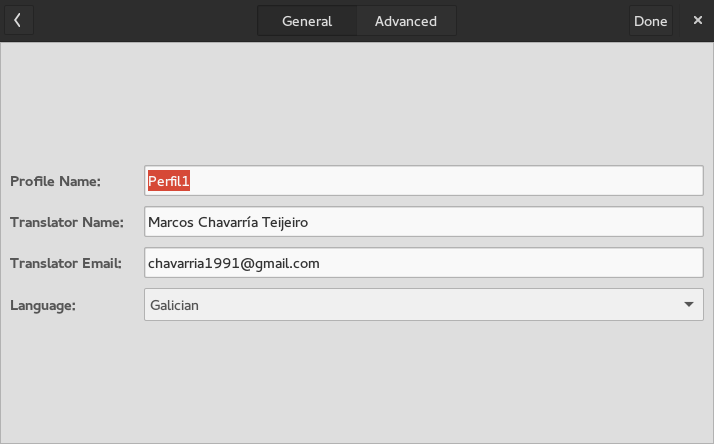
\includegraphics[width=\textwidth]{img/panel_pefil_xeral.png}
    \caption{Diagrama de Clases do módulo ficheiros}
    \label{fig:dia_class:files}
\end{figure}

\begin{figure}[h!]
    \centering
    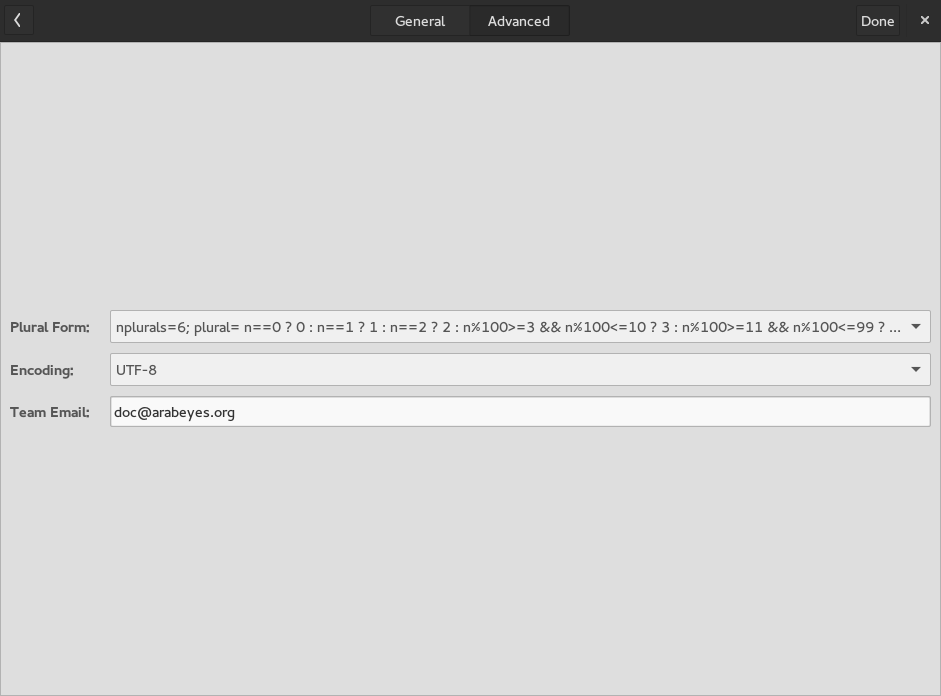
\includegraphics[width=\textwidth]{img/panel_perfil_avanzado.png}
    \caption{Diagrama de Clases do módulo ficheiros}
    \label{fig:dia_class:files}
\end{figure}

\begin{figure}[h!]
    \centering
    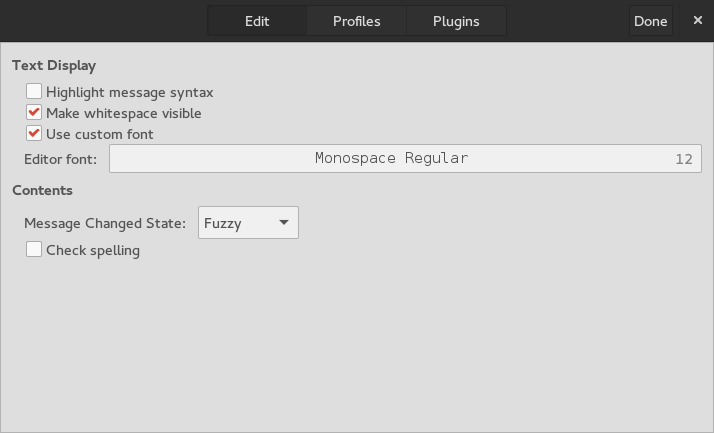
\includegraphics[width=\textwidth]{img/panel_preferencias_edicion.png}
    \caption{Diagrama de Clases do módulo ficheiros}
    \label{fig:dia_class:files}
\end{figure}

\begin{figure}[h!]
    \centering
    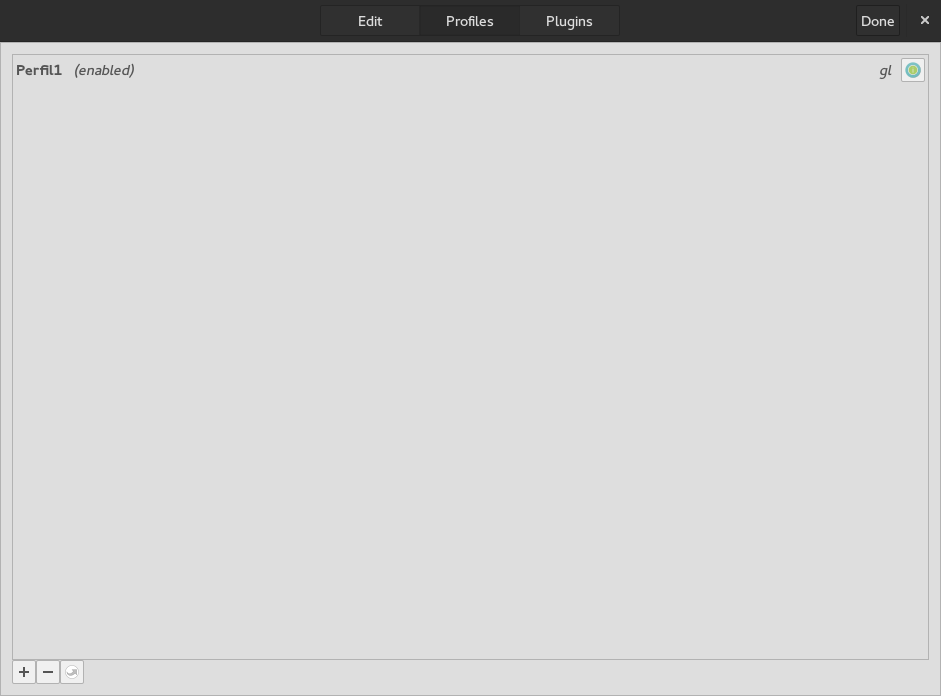
\includegraphics[width=\textwidth]{img/panel_preferencias_perfiles.png}
    \caption{Diagrama de Clases do módulo ficheiros}
    \label{fig:dia_class:files}
\end{figure}

\begin{figure}[h!]
    \centering
    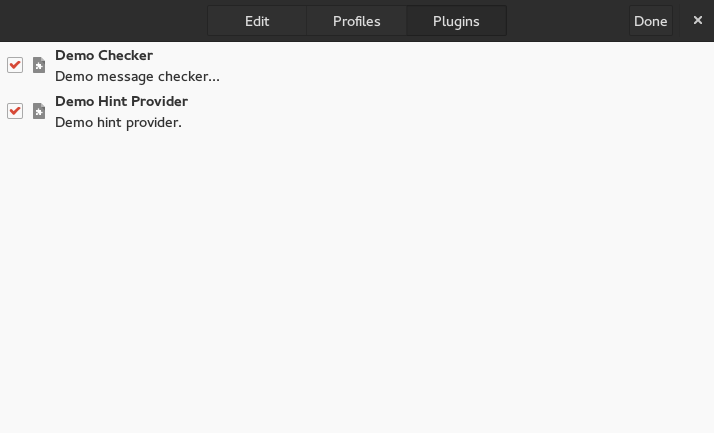
\includegraphics[width=\textwidth]{img/panel_preferencias_plugins.png}
    \caption{Diagrama de Clases do módulo ficheiros}
    \label{fig:dia_class:files}
\end{figure}


\section{Navegación e Busca a través do documento}

\section{Preferencias}

\subsection{Módulo de Perfiles}

\section{Plugins}
